\documentclass[
	12pt, % Default font size, values between 10pt-12pt are allowed
	%letterpaper, % Uncomment for US letter paper size
	%english, % Uncomment for Spanish
]{article}


%These tell TeX which packages to use.
\usepackage{array,epsfig}
\usepackage{amsmath}
\usepackage{amsfonts}
\usepackage{amssymb}
\usepackage{amsxtra}
\usepackage{amsthm}
\usepackage{mathrsfs}
\usepackage{color}
\usepackage[margin=2cm,top=2.5cm,headheight=16pt,headsep=0.1in,heightrounded]{geometry}
\usepackage{fancyhdr}
\pagestyle{fancy}
\usepackage{tikz}
\usepackage{graphics}
\usepackage{float}
\usepackage{listings}

%Here I define some theorem styles and shortcut commands for symbols I use often
\theoremstyle{definition}
\newtheorem{defn}{Definition}
\newtheorem{thm}{Theorem}
\newtheorem{cor}{Corollary}
\newtheorem*{rmk}{Remark}
\newtheorem{lem}{Lemma}
\newtheorem*{joke}{Joke}
\newtheorem{ex}{Example}
\newtheorem*{soln}{Solution}
\newtheorem{prop}{Proposition}

\newcommand{\lra}{\longrightarrow}
\newcommand{\ra}{\rightarrow}
\newcommand{\surj}{\twoheadrightarrow}
\newcommand{\graph}{\mathrm{graph}}
\newcommand{\bb}[1]{\mathbb{#1}}
\newcommand{\Z}{\bb{Z}}
\newcommand{\Q}{\bb{Q}}
\newcommand{\R}{\bb{R}}
\newcommand{\E}{\bb{E}}
\newcommand{\C}{\bb{C}}
\newcommand{\N}{\bb{N}}
\newcommand{\Pe}{\bb{P}}
\newcommand{\M}{\mathbf{M}}
\newcommand{\m}{\mathbf{m}}
\newcommand{\MM}{\mathscr{M}}
\newcommand{\HH}{\mathscr{H}}
\newcommand{\Om}{\Omega}
\newcommand{\Ho}{\in\HH(\Om)}
\newcommand{\bd}{\partial}
\newcommand{\del}{\partial}
\newcommand{\bardel}{\overline\partial}
\newcommand{\textdf}[1]{\textbf{\textsf{#1}}\index{#1}}
\newcommand{\img}{\mathrm{img}}
\newcommand{\ip}[2]{\left\langle{#1},{#2}\right\rangle}
\newcommand{\inter}[1]{\mathrm{int}{#1}}
\newcommand{\exter}[1]{\mathrm{ext}{#1}}
\newcommand{\cl}[1]{\mathrm{cl}{#1}}
\newcommand{\ds}{\displaystyle}
\newcommand{\vol}{\mathrm{vol}}
\newcommand{\cnt}{\mathrm{ct}}
\newcommand{\osc}{\mathrm{osc}}
\newcommand{\LL}{\mathbf{L}}
\newcommand{\UU}{\mathbf{U}}
\newcommand{\support}{\mathrm{support}}
\newcommand{\AND}{\;\wedge\;}
\newcommand{\OR}{\;\vee\;} 
\newcommand{\Oset}{\varnothing}
\newcommand{\st}{\ni}
\newcommand{\wh}{\widehat}
\newcommand{\vect}[1]{\overrightarrow{#1}}

%Pagination stuff.
%\setlength{\oddsidemargin}{0in}
%\setlength{\evensidemargin}{0in}
%\setlength{\textheight}{9.in}
%\setlength{\textwidth}{6.5in}
%\cfoot{page \thepage}
%\lhead{MEU359 - Proba-Stat}
%\rhead{TP}
%\pagestyle{fancy}



\newcommand{\maketitletwo}{
\begin{center}
    \Large{\textbf{Academic Writing Sample}
        
        Estimation of the Eucalyptus tree heights} % Name of course here
    \vspace{5pt}
    
    \normalsize{Charlotte Ayrault  % Your name here
    
    \today}        % Change to due date if preferred
    \vspace{15pt}
\end{center}}    

%----------------------------------------------------------------------------------------

\begin{document}

\maketitletwo 


\section{Introduction}
We are looking at a way to estimate the height of eucalyptus trees. One way to solve this problem is to calculate the height from another physical characteristic of the tree. We have a database of 1,400 samples from the circumference of the tree's trunk measured at 1.3 meter from the ground and the actual height of the tree. 

\smallskip
I have been asked to verify that the measure of the circumference is a good indicator of the height of the eucalyptus trees and to provide the equation based on 2 statistical models; the simple linear regression (SLR) and the multiple linear regression (MLR).


\smallskip
This problem illustrates how a simple measure can help eucalyptus farmer to identify which tree should be cut depending on the final product issued from the tree.

\medskip
This academic writing is based on a work performed by myself for the Statistic course at Saclay University in May 2022.

\section{Simple Linear Regression}

Simple linear regression provides a means to model with a straight line relationship between two variables. In order to use this model, some conditions should be verified on the data set:
\begin{enumerate}
    \item Homogeneity of the variance: the value of the error in our prediction doesn't change too much across the values of the independent variable. 

    \item Independence of observations: the data set were collected using statistically valid sampling methods. There is no hidden relationships among observations like choosing specific trees.

    \item Normality: The collected data follows a normal distribution. 
    
    \item The relationship between the independent and dependent variable is linear: the line of best fit through the data points is a straight line (rather than a curve or some sort of grouping factor).
\end{enumerate} 

Figure \ref{fig:regression} is a scatter of dataset.

\begin{figure}[H]
	\includegraphics[scale=1]{dataset.jpg}
    \caption{Data set}
    \label{fig:regression}
\end{figure}


We can clearly see that the scatter plot is compact (no point completely outside the others), this satisfies the condition 1. It is also arranged along a straight line, this satisfies the condition 4. We can only assume that the collected data are unbias to satisfies the condition 2. Condition 3 is verified on the following figures \ref{fig:Circumference} and \ref{fig:Height}. The figures trace the distribution of the circumferences and the heights and their average. It shows that the data follows a normal distribution.


\begin{figure}[H]
    \centering
    \begin{minipage}{0.45\textwidth}
        \centering
            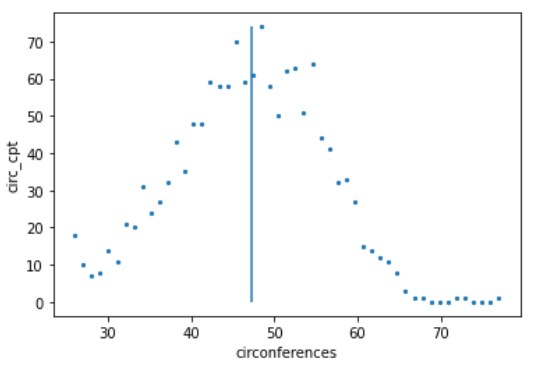
\includegraphics[scale=0.5]{circ_normale.jpg}
            \caption{Circumference}
            \label{fig:Circumference}
    \end{minipage}\hfill
    \begin{minipage}{0.45\textwidth}
        \centering
        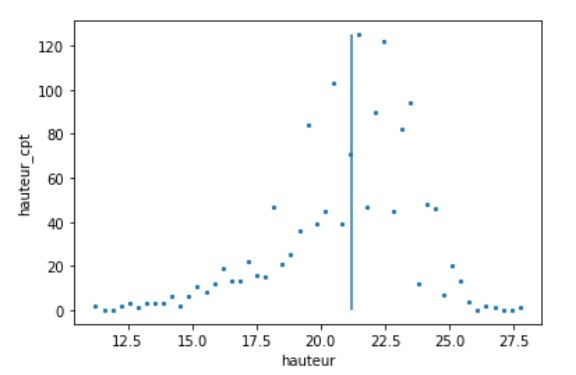
\includegraphics[scale=0.5]{hauteur_normale.jpg}
        \caption{Height}
        \label{fig:Height}
    \end{minipage}
\end{figure}


Therefore the Simple Linear Regression can be a good candidate to model this problem as it aims to define the equation of a line. 


The Simple Linear Regression model consists to suppose that a variable $y$ can be expressed linearly in function of a variable $x$ with a sample random variation noted $\epsilon$. The variation is called "residual" or "noise". 

$$
\forall i \in {1, . . . , n}, y_i = \beta_1 + \beta_2x_i + \epsilon_i
$$

Variables $x_i$ and $y_i$ are observed data, when the value $\beta_1$ and $\beta_2$ are unknown.
We are then looking for a straight line with the equation $y = \beta_1 + \beta_2x$ that provides the relationship between $x$ and $y$ and minimizes $\epsilon$ in a certain way.

One way to solve the problem is to find the value of $\beta_1$ et $\beta_2$ obtained by minimizing the sum of squared residuals.
$$
\varphi(\beta_1, \beta_2) = \sum_{i=1}^{n}{\epsilon_i^2} = \sum_{i=1}^{n}{(y_i - \beta_1 - \beta_2x_i)^2}
$$

\section{Calculation of $\beta_1$ and $\beta_2$}
The way to minimum of the function $\varphi(\beta_1, \beta_2)$ is to calculate the derivative of the function $\varphi(\beta_1, \beta_2)$ with respect to $\beta_1$ and $\beta_2$ and then to find the values where the 2 derivatives are equal to 0.

\bigskip
The first derivative is
$$
\frac{\partial \varphi(\beta_1, \beta_2)}{\beta_1} = \frac{\sum_{i=1}^{n}{(Y_i - \beta_1 - \beta_2x_i)^2}}{\beta_1} 
$$
$$
= \frac{\sum_{i=1}^{n}{Y_i^2 - \beta_1Y_i - \beta_2x_iY_i -\beta_1Y_i + \beta_1^2 + \beta_1\beta_2x_i - \beta_2x_iY_i + \beta_2x_i\beta_1 +\beta_2^2x_i^2}}{\beta_1}
$$
$$
= \sum_{i=1}^{n}{-Y_i -Y_i +2\beta_1 +\beta_2x_i+\beta_2x_i} = 2 \sum_{i=1}^{n}{-Y_i+\beta_2x_i+\beta_1}
$$

\bigskip
The second derivative is
$$
\frac{\partial \varphi(\beta_1, \beta_2)}{\beta_2} = \frac{\sum_{i=1}^{n}{(Y_i - \beta_1 - \beta_2x_i)^2}}{\beta_2}
$$
$$
= \frac{\sum_{i=1}^{n}{Y_i^2 - \beta_1Y_i - \beta_2x_iY_i -\beta_1Y_i + \beta_1^2 + \beta_1\beta_2x_i - \beta_2x_iY_i + \beta_2x_i\beta_1 +\beta_2^2x_i^2}}{\beta_2}
$$
$$
= \sum_{i=1}^{n}{-x_iY_i+\beta_1x_i-x_iY_i + \beta_1x_i+2\beta_2x_i^2} = 2 \sum_{i=1}^{n}{x_i(-Y_i+\beta_2x_i+\beta_1)}
$$

We are looking for the values $\beta_1$ and $\beta_2$ that nullifies the following system.

$$
\left\{
\begin{array}{l}
\sum_{i=1}^{n}{x_i(-Y_i+\beta_2x_i+\beta_1)} = 0 \\
\sum_{i=1}^{n}{-Y_i+\beta_2x_i+\beta_1} = 0
\end{array}
\right.
$$
$$
\left\{
\begin{array}{l l}
\sum_{i=1}^{n}{-Y_ix_i}+\sum_{i=1}^{n}{\beta_2x_i^2}+\sum_{i=1}^{n}{\beta_1x_i} = 0 & (1)\\
\sum_{i=1}^{n}{-Y_i} +\sum_{i=1}^{n}{\beta_2x_i}+\sum_{i=1}^{n}{\beta_1} = 0 & (2)
\end{array}
\right.
$$
$$
\left\{
\begin{array}{l l}
\sum_{i=1}^{n}{-Y_ix_i}+\beta_2\sum_{i=1}^{n}{x_i^2}+\beta_1\sum_{i=1}^{n}{x_i} = 0 & (1)\\
\sum_{i=1}^{n}{-Y_i} +\beta_2\sum_{i=1}^{n}{x_i}+n\beta_1 = 0 & (2)
\end{array}
\right.
$$

\bigskip
We calculate $(3) = n(1)-(2)\sum_{i=1}^{n}{x_i}$
$$
\left\{
\begin{array}{l l}
n\sum_{i=1}^{n}{-Y_ix_i}+n\beta_2\sum_{i=1}^{n}{x_i^2}+\sum_{i=1}^{n}{Y_i}\sum_{i=1}^{n}{x_i} -\beta_2\left(\sum_{i=1}^{n}{x_i}\right)^2 = 0 & (3)\\
\sum_{i=1}^{n}{-Y_i} +n\beta_2\sum_{i=1}^{n}{x_i}+n\beta_1 = 0 & (2)
\end{array}
\right.
$$
$$
\left\{
\begin{array}{l l}
-n\sum_{i=1}^{n}{Y_ix_i} + \sum_{i=1}^{n}{Y_i}\sum_{i=1}^{n}{x_i} = \beta_2\left(\sum_{i=1}^{n}{x_i}\right)^2 -n\beta_2\sum_{i=1}^{n}{x_i^2}  & (3)\\
\sum_{i=1}^{n}{-Y_i} +n\beta_2\sum_{i=1}^{n}{x_i}+n\beta_1 = 0 & (2)
\end{array}
\right.
$$
$$
\left\{
\begin{array}{l l}
\beta_2 = \frac{\sum_{i=1}^{n}{Y_i}\sum_{i=1}^{n}{x_i}-n\sum_{i=1}^{n}{Y_ix_i}}{\left(\sum_{i=1}^{n}{x_i}\right)^2 -n\sum_{i=1}^{n}{x_i^2}}  & (3)\\
\beta_1 = \frac{1}{n}(\sum_{i=1}^{n}{Y_i} - n\beta_2\sum_{i=1}^{n}{x_i}) & (2)
\end{array}
\right.
$$

\bigskip
To obtain the following values.

$$
\left\{
\begin{array}{l l}
\beta_2 = \frac{\sum_{i=1}^{n}{Y_i}\sum_{i=1}^{n}{x_i}-n\sum_{i=1}^{n}{Y_ix_i}}{\left(\sum_{i=1}^{n}{x_i}\right)^2 -n\sum_{i=1}^{n}{x_i^2}}  & (3)\\
\beta_1 = \frac{\sum_{i=1}^{n}{x_i}\sum_{i=1}^{n}{x_iY_i}-\sum_{i=1}^{n}{x_i^2}\sum_{i=1}^{n}{Y_i}}{\left(\sum_{i=1}^{n}{x_i}\right)^2 -n\sum_{i=1}^{n}{x_i^2}} & (2)
\end{array}
\right.
$$

The values can be calculated using a Python program (see appendix A). I obtain $\beta_1 =  9.037475668452768$  et $\beta_2 = 0.257137855007109$ and

\begin{itemize}
    \item Average of the $\epsilon_i$: -3.603610217941441e-11
    \item Sum of squared $\epsilon_i$ : 19.492804231375466
\end{itemize}

The straight line is shown on figure \ref{fig:regression simple}

\begin{figure}[H]
	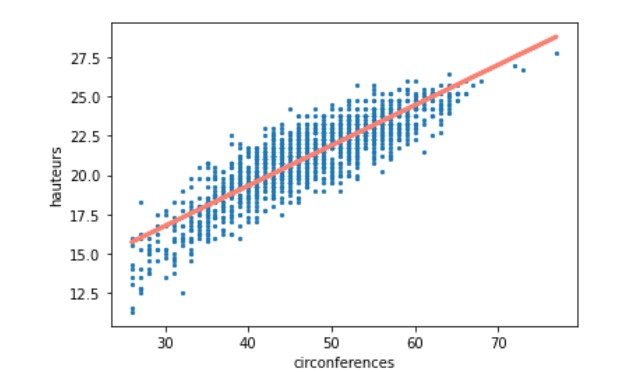
\includegraphics[scale=0.8]{regression_simple.jpg}
    \caption{Simple Linear Regression}
    \label{fig:regression simple}
\end{figure}


We can see that for the medium values of the circumferences the Linear model is accurate, for the low and high values of the circumferences the line over-estimates the height. Adding a 
    
\pagebreak
\section{Multiple Linear Regression}


The Multiple Linear Regression Model is used when the relation is between two or more explanatory variables and a response variable.
$$
\forall i \in \{1,\dots,n\}, Y_i = \beta_1 + \beta_2x_2 + \beta_3x_3 + \ldots + \beta_nx_n + \epsilon_i
$$

Where the $b_ix_i$ are called the regression coefficients of the regression. 

\bigskip
On our problem, with only have one explanatory variable; the circumference of the eucalyptus tree. So a way to apply the Multiple Linear Model is to use polynomial values of the variable to generate "new" explanatory variables. 

\medskip
We try to correct the model by lightly lowered both side of the straight line. Based on the Simple Linear Model, we need to find which polynomial could provide the best correction. Polynomials greater than 1 may provide a too aggressive correction. Therefore, we need to propose a polynomial less than 1. Let's try $\sqrt{x}$, as lesser value could be too aggressive too. Let try the following model. 

$$
\forall i \in \{1,\dots,n\}, Y_i = \beta_1 + \beta_2x_i + \beta_3\sqrt{x_i} + \epsilon_i
$$

The method used to calculate the $\beta_i$ for the Simple Linear Model cannot be used. A more generic resolution method should be used. The Multiple Linear Regression can be rewritten using matrices. 

$$
Y = X\beta + \epsilon
$$

With 
\begin{itemize}
    \item $Y$ a column vector of size $n \times 1$ build as $\begin{pmatrix} y_1 \\ y_2 \\ \vdots \\ y_n \end{pmatrix}$, 
    \item $X$ a matrix of size $n \times 3$ build as $\begin{pmatrix} 1 & x_1 & \sqrt{x_1} \\ 1 & x_2 & \sqrt{x_2}  \\ \vdots & \vdots & \vdots \\ 1 & x_n & \sqrt{x_n}  \end{pmatrix}$ 
    \item $\beta = \begin{pmatrix} \beta_1 \\ \beta_2 \\ \beta_3 \end{pmatrix}$
    \item $\epsilon$ column vectors of size $n \times 1$, $\begin{pmatrix} \epsilon_1 \\ \epsilon_2 \\ \vdots \\ \epsilon_n \end{pmatrix}$
\end{itemize}

As for the Simple Linear Regression we try to minimize

$$
\varphi(\beta) = \sum_{i=1}^{n}{\epsilon_i^2} = \sum_{i=1}^{n}{(y_i - \beta_1 - \beta_2x_i - \sqrt{\beta_3})^2} = \lVert Y - X\beta \rVert^2
$$

We note $F$ the vector space based on the column of $X$. $F = Vect(1,x,\sqrt{x})$. A vector $z$ belongs to $F$ if and only if there exists $\beta$ such that $z = X\beta'$. The problem to solve is to find the value $\beta$ that minimize the function $\varphi(\beta)$ for the given values $Y$ and $X$. 

\bigskip
Looking for minimizing $\lVert Y - X\beta \rVert^2$, is identical than finding the point from the vector space $F$ which is at the closest euclidian distance from $Y$. This is the definition of the orthogonal projection of $Y$ on $F$. As $z \in F$, if and only if $z = X\beta'$, we are looking for $\beta$ such that $X\beta = P_F(Y)$ where $P_F$ is the orthogonal projection of $Y$ on $z$.  

\bigskip
To find the minima regarding $\beta$, we can derive the expression with respect to $\beta$ and nullifies the result. This is done using the fact that $\sum_{i=1}^{n}{(Y-X\beta)^2} = (Y-X\beta)^t(Y-X\beta)$ where $X^t$ is the transpose on $X$.

$$
(Y-X\beta)^t(Y-X\beta) = (Y^t-\beta^tX^t)(Y-X\beta) = Y^tY-Y^tX\beta - \beta^tX^tY + \beta^tX^tX\beta
$$
et
$$
\frac{\partial (Y-X\beta)^t(Y-X\beta) }{\partial \beta} = -Y^tX + \beta^tX^tX
$$

We are looking for $\beta$ such that
$$
-Y^tX + \hat{\beta}^tX^tX = 0
$$
$$
\beta^tX^tX)^t = (-Y^tX)^t
$$
So
$$
\beta = (X^tX)^{-1}X^tY
$$

The values can be calculated using a Python program (see appendix B)

$$\beta = \begin{pmatrix} -24.35200327 \\  -0.48294547 \\ 9.98688814 \end{pmatrix}$$

\begin{figure}[H]
	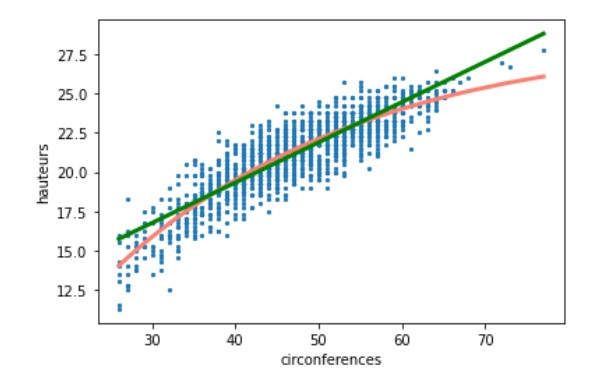
\includegraphics[scale=1]{regression_multiple.jpg}
    \caption{Regression multiple}
    \label{fig:Regression multiple}
\end{figure}


\begin{itemize}
    \item Average of the $\epsilon_i$ : 1.0692449957862278e-13
    \item Sum of the squared $\epsilon_i$ : 19.32298986873724
\end{itemize}
\bigskip
The new values are closed but better than the those of the Simple Linear Regression.



\bigskip
The Python program also calculates the values of $\beta$ for the Simple Linear Regression using $X = \begin{pmatrix} 1 & x_1 \\ 1 & x_2 \\ \vdots & \vdots \\ 1 & x_n  \end{pmatrix}$. I found the same values of $\beta$ than for the Simple Linear Regression.

\pagebreak
\section{Appendices. Python code}

\subsection{Simple Linear Regression}
\begin{lstlisting}[language=Python]
import csv
import matplotlib.pyplot as plt
import numpy as np
from scipy.stats import t
import os

# lecture fichier Eucalypcus
file = open(os.getcwd()+"\\Eucaliptus.csv")
csvreader = csv.reader(file)
next(csvreader)

circs = np.empty([0])
hauteurs = np.empty([0])

for row in csvreader:
    c = float(row[1])
    h = float(row[2])
    circs = np.append(circs,c)
    hauteurs = np.append(hauteurs,h)

max_c = np.amax(circs)
min_c = np.amin(circs)
max_h = np.amax(hauteurs)
min_h = np.amin(hauteurs)

pas = 50

# circs
circs_cpt = np.zeros(pas+1)
diff_c = max_c - min_c
axis_x = min_c + np.arange(0,pas+1)*diff_c/pas
for c in circs:
    index = int((c - min_c)*pas/diff_c)
    circs_cpt[index] += 1

plt.scatter(axis_x, circs_cpt,s=5)
plt.vlines(x = np.mean(circs), ymin = 0, ymax = np.amax(circs_cpt)) 
plt.ylabel("circ_cpt");
plt.xlabel("circonferences")
plt.show()


# hauteurs
hauteurs_cpt = np.zeros(pas+1)
diff_h = max_h - min_h
axis_h = min_h + np.arange(0,pas+1)*diff_h/pas
for h in hauteurs:
    index = int((h - min_h)*pas/diff_h)
    hauteurs_cpt[index] += 1

plt.scatter(axis_h, hauteurs_cpt,s=5)
plt.vlines(x = np.mean(hauteurs), ymin = 0, ymax = np.amax(hauteurs_cpt)) 
plt.ylabel("hauteur_cpt");
plt.xlabel("hauteur")
plt.show()

# Calcul des betas
xi = 0.0
yi = 0.0
xi2 = 0.0
xiyi= 0.0
circs = np.empty([0])
hauteurs = np.empty([0])

for row in csvreader:
    c = float(row[1])
    h = float(row[2])
    xi += c
    yi += h
    xiyi += c*h
    xi2 += c**2
    circs = np.append(circs,c)
    hauteurs = np.append(hauteurs,h)

    n = circs.size
    beta1 = (xi2*yi - xi*xiyi)/(n*xi2-xi**2)
    beta2 = (n*xiyi - xi*yi)/(n*xi2-xi**2)
    print(f"beta1: {beta1}, beta2: {beta2}")
    
    y = beta1+beta2*circs
    
    plt.scatter(circs, hauteurs,s=5)
    plt.plot(circs, y, color='salmon', linewidth=3)
    plt.xlabel("circonferences");
    plt.ylabel("hauteurs")
    plt.show()
    
    print(f"Moyenne de espilon: {np.sum(y-hauteurs)/n}")
\end{lstlisting}


\subsection{Multiple Linear Regression}

\begin{lstlisting}[language=Python]
    # lecture fichier Eucalypcus
    file = open(os.getcwd()+"\\Eucaliptus.csv")
    csvreader = csv.reader(file)
    next(csvreader)
    
    circs = np.empty([0,3], float)
    circs1 = np.empty([0,2], float)
    circs2 = np.empty([0,5], float)
    hauteurs = np.empty([0])
    
    for row in csvreader:
        c = float(row[1])
        h = float(row[2])
        circs  = np.append(circs,[(1.0,c,np.sqrt(c))],axis=0)     # regression multiple ordre 2
        circs1 = np.append(circs1,[(1.0,c)],axis=0)               # regression simple
        hauteurs = np.append(hauteurs,h)
    
    file.close()

def calcule_beta(X, Y):
    XT = X.transpose()
    A = np.matmul(XT,X)
    A_inv = np.linalg.inv(A)
    B = np.matmul(XT,Y)
    beta = np.matmul(A_inv,B)
    return beta

print(f"Beta: {calcule_beta(circs, hauteurs)}")
print(f"Beta: {calcule_beta(circs1, hauteurs)}") # meme resultats que la regression lineaire simple 

beta = calcule_beta(circs, hauteurs)
# Tri par hauteurs pour tracer proprement la courbe
circs_sort = circs[circs[:, 1].argsort()]
y = beta[0]+beta[1]*circs_sort[:,[1]]+beta[2]*circs_sort[:,[2]]

beta1 = calcule_beta(circs1, hauteurs)
print(f"Beta multiple: {beta}")

beta1 = calcule_beta(circs1, hauteurs)
# Tri par hauteurs pour tracer proprement la courbe
circs1_sort = circs1[circs1[:, 1].argsort()]
y1 = beta1[0]+beta1[1]*circs1_sort[:,[1]]
print(f"Beta simple: {beta1}") # meme resultats que la regression lineaire simple 


plt.scatter(circs[:,[1]], hauteurs,s=5)
plt.plot(circs_sort[:,[1]], y, color='salmon', linewidth=2)   # regression lineaire multiple
plt.plot(circs1_sort[:,[1]], y1, color='green', linewidth=2)  # regression lineaire simple
plt.xlabel("circonferences")
plt.ylabel("hauteurs")
plt.show()

res = 0
for i in range(hauteurs.size):
    h = beta[0] + beta[1]*circs[i,1] + beta[2]*circs[i,2]
    res = res + np.power(hauteurs[i] - h,2) 
res1 = 0
for i in range(hauteurs.size):
    h1 = beta1[0] + beta1[1]*circs1[i,1]
    res1 = res1 + np.power(hauteurs[i] - h1,2) 

print(f"Moyenne de espilon: {(np.sum(y)-np.sum(hauteurs))/n}")
print(f"risque quadratique: {h}")
print(f"Moyenne de espilon: {(np.sum(y1)-np.sum(hauteurs))/n}")
print(f"risque quadratique: {h1}")

\end{lstlisting}


\end{document}

